\documentclass{report}
\usepackage[latin1]{inputenc}
\usepackage[T1]{fontenc}
\usepackage{graphicx}
\usepackage{algorithm}
\usepackage{algorithmic}
\usepackage[margin=0.5in]{geometry}

\title{Projet de Robotique : Comportement du Robot}
\author{Groupe 7}
\begin{document}

\maketitle

\chapter{Version 1}

\section{Comportement}
\begin{algorithm}
\caption{Comportement}
\begin{algorithmic}
\WHILE{true}
\STATE D\'etecter personnes
\STATE D\'etecter groupes
\STATE Rejoindre le groupe choisi
\STATE Attendre 5 minutes
\ENDWHILE
\end{algorithmic}
\end{algorithm}

\begin{center}
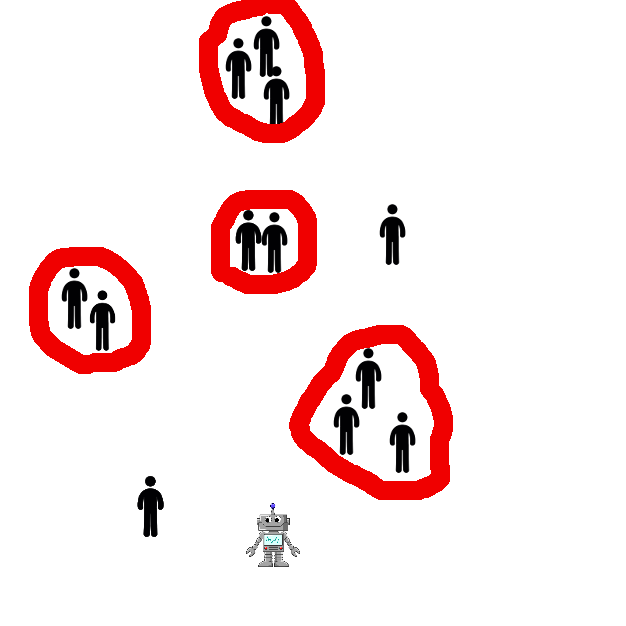
\includegraphics[scale=0.6]{v1_action_robot.png}
\end{center}
\subsection{Les personnes}

C'est le noeud : moving\_person\_detector qui d\'etecte les personnes.

\subsection{Les groupes}

On consid\`ere comme groupe, un ensemble d'au moins deux personnes, o\`u chaque
personne \`a un voisin \`a moins d'un metre. C'est le noeud group\_detector qui
d\'etecte les groupes.\\
Si il ' y a au moins un groupe, le groupe vers lequel se d\'eplace le robot est
le groupe le plu proche du robot. Pour \'eviter que le robot reste devant le
m\^eme groupe, le robot doit se d\'eplacer vers un groupe qui se trouve \`a une
distance minimale de e. C'est le noeud group\_detector qui choisi le
groupe \`a rejoindre.

\section{architecture}

\begin{center}
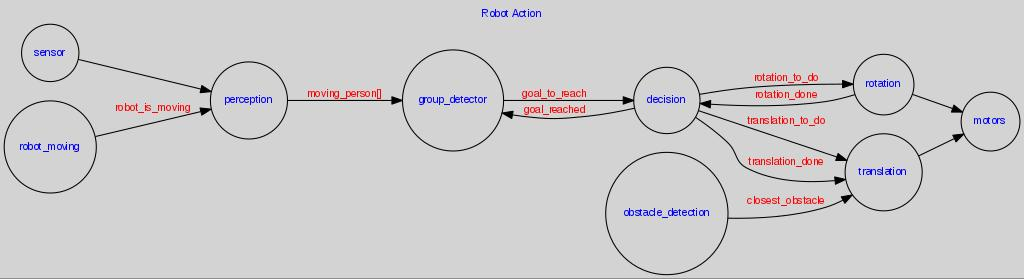
\includegraphics[scale=0.6]{automata.jpg}
\end{center}

\section{Partage du travail}

\begin{itemize}
\item Georges : Communication detect\_person detect\_group (envoie tableau
  de coordonn\'ees)
\item Maxence : D\'etection de groupe
  \item Thaqif : Choix du groupe \`a rejoindre + envoie du goal\_to\_reach
\end{itemize}
\end{document}
